% beamer for weekly report
% Created by Zihan on 2023-06-22

% turn off sans-serif math
\documentclass[11pt]{beamer}

% Packages
% \Sum
\usepackage{amsmath}
% \coloneqq
\usepackage{mathtools}
% bookmark
\usepackage{bookmark}

% theme
\usetheme{default}
\usefonttheme{serif}

% title
\title{Weekly Report}

% author
\author{Zihan}

% date
\date{\today}

% Document
\begin{document}

% no title frame

% first page
% Talk about the paper supervisor asked me to read

\begin{frame}
    \frametitle{Co-Clustering to Reveal Salient Facial Features for Expression Recognition}
    \begin{itemize}
        \item \textbf{Proposal} Use co-clustering to select features that can be used to classify facial expressions
        \item \textbf{Method}
              \begin{itemize}
                  \item Use Gabor filter to extract features from facial images
                  \item Use co-clustering to attain a subset of features and samples
                        % 计算每个co-cluster对应的samples和某个class契合的程度
                  \item Find the probability that a co-cluster is related to a certain class
                  \item Features with high probability are selected
              \end{itemize}
    \end{itemize}
    % insert a picture 'khan.png'
    \begin{figure}[htbp]
        \centering
        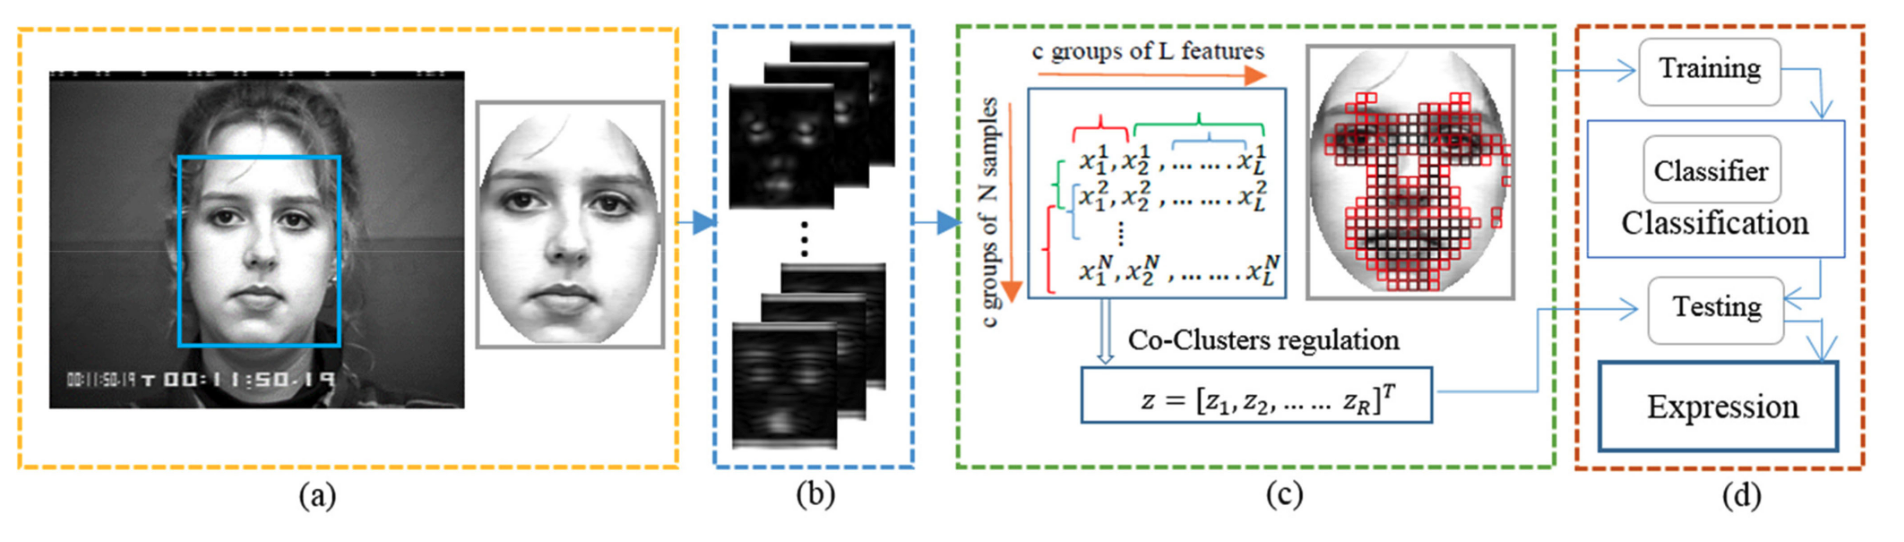
\includegraphics[width=\textwidth]{khan.png}
        \caption{Khan et al. 2017}
    \end{figure}
\end{frame}

% second page
% My proposal according to the paper

\begin{frame}
    \frametitle{My Proposal}
    \begin{itemize}
        \item Word-embedding or $n$-gram to extract features from text
        \item (Maybe) Generate more features from the results above
        \item Use co-clustering to attain a subset of features and samples
        \item Select features that are related to a certain class most
    \end{itemize}
\end{frame}

% third page
% I find another very high-quality paper about the feature selection in general case, which is 2017 best paper of ICML

\begin{frame}
    \frametitle{Best Paper of ICML 2017}
    \begin{itemize}
        \item \textbf{Title} Understanding Black-box Predictions via Influence Functions
        \item \textbf{Authors} Pang Wei Koh, Percy Liang
        \item \textbf{Introduction} This paper uses influence function to measure the importance of each training sample and feature. 
    \end{itemize}
\end{frame}

\end{document}
